\documentclass[a4paper, 12pt, oneside, titlepage]{article} %{\parskip}
\usepackage[top=2.54cm, bottom=2.54cm, left=3cm, right=2cm]{geometry}
\usepackage[utf8]{inputenc}
\usepackage[czech]{babel}
\usepackage[T1]{fontenc}
\usepackage{graphicx}
\usepackage{booktabs}
\usepackage{tabularx}
\usepackage{array}
\usepackage{indentfirst}
\usepackage{multicol}
\usepackage{titlesec}
\usepackage{mathtools}
\usepackage{esvect}

\usepackage{url}
\usepackage{caption}
\usepackage{subfig}
\usepackage[section]{placeins}
\usepackage{pdfpages}



\hyphenation{po-ly-gon desk-to-po-vá}

\newcommand{\tg}{\mathop{\rm tg}\nolimits}
\newcommand{\arctg}{\mathop{\rm arctg}\nolimits}
\newtheorem{defin}{Definice}

\begin{document}

%\pagestyle{empty}
\setcounter{page}{1}   % nastaví čítač stránek znovu od jedné
\pagenumbering{arabic} % číslování arabskými
\thispagestyle{empty}

\begin{center}

\large

\v{C}eské vysoké učení technické v~Praze

\medskip

Fakulta stavební
\medskip

Katedra geomatiky

\vfill
\centerline{\mbox{
\includegraphics[scale=1.3]{obrazky/symbol_cvut_konturova_verze.jpg}} }


{\bf\Large Technická zpráva}

\vfill

{\bf\LARGE\bfseries Algoritmy v digitální kartografii}

\vfill

{\bf\Large Úloha č. 3: Digitální model terénu}


\vfill



\vfill
\vspace{5mm}

\begin{tabular}{c}

{\bf Bc. Pane Kuzmanov}\\
\noalign{\vspace{2mm}}
{\bf Bc. František Mužík}\\
\noalign{\vspace{10mm}}

Studijní program: Geodézie a kartografie \\
\noalign{\vspace{2mm}}

Specializace: Geomatika\\

\end{tabular}


\vfill

% Zde doplňte rok
Praha 2021

\end{center}

%---------------------------------------------------------------------
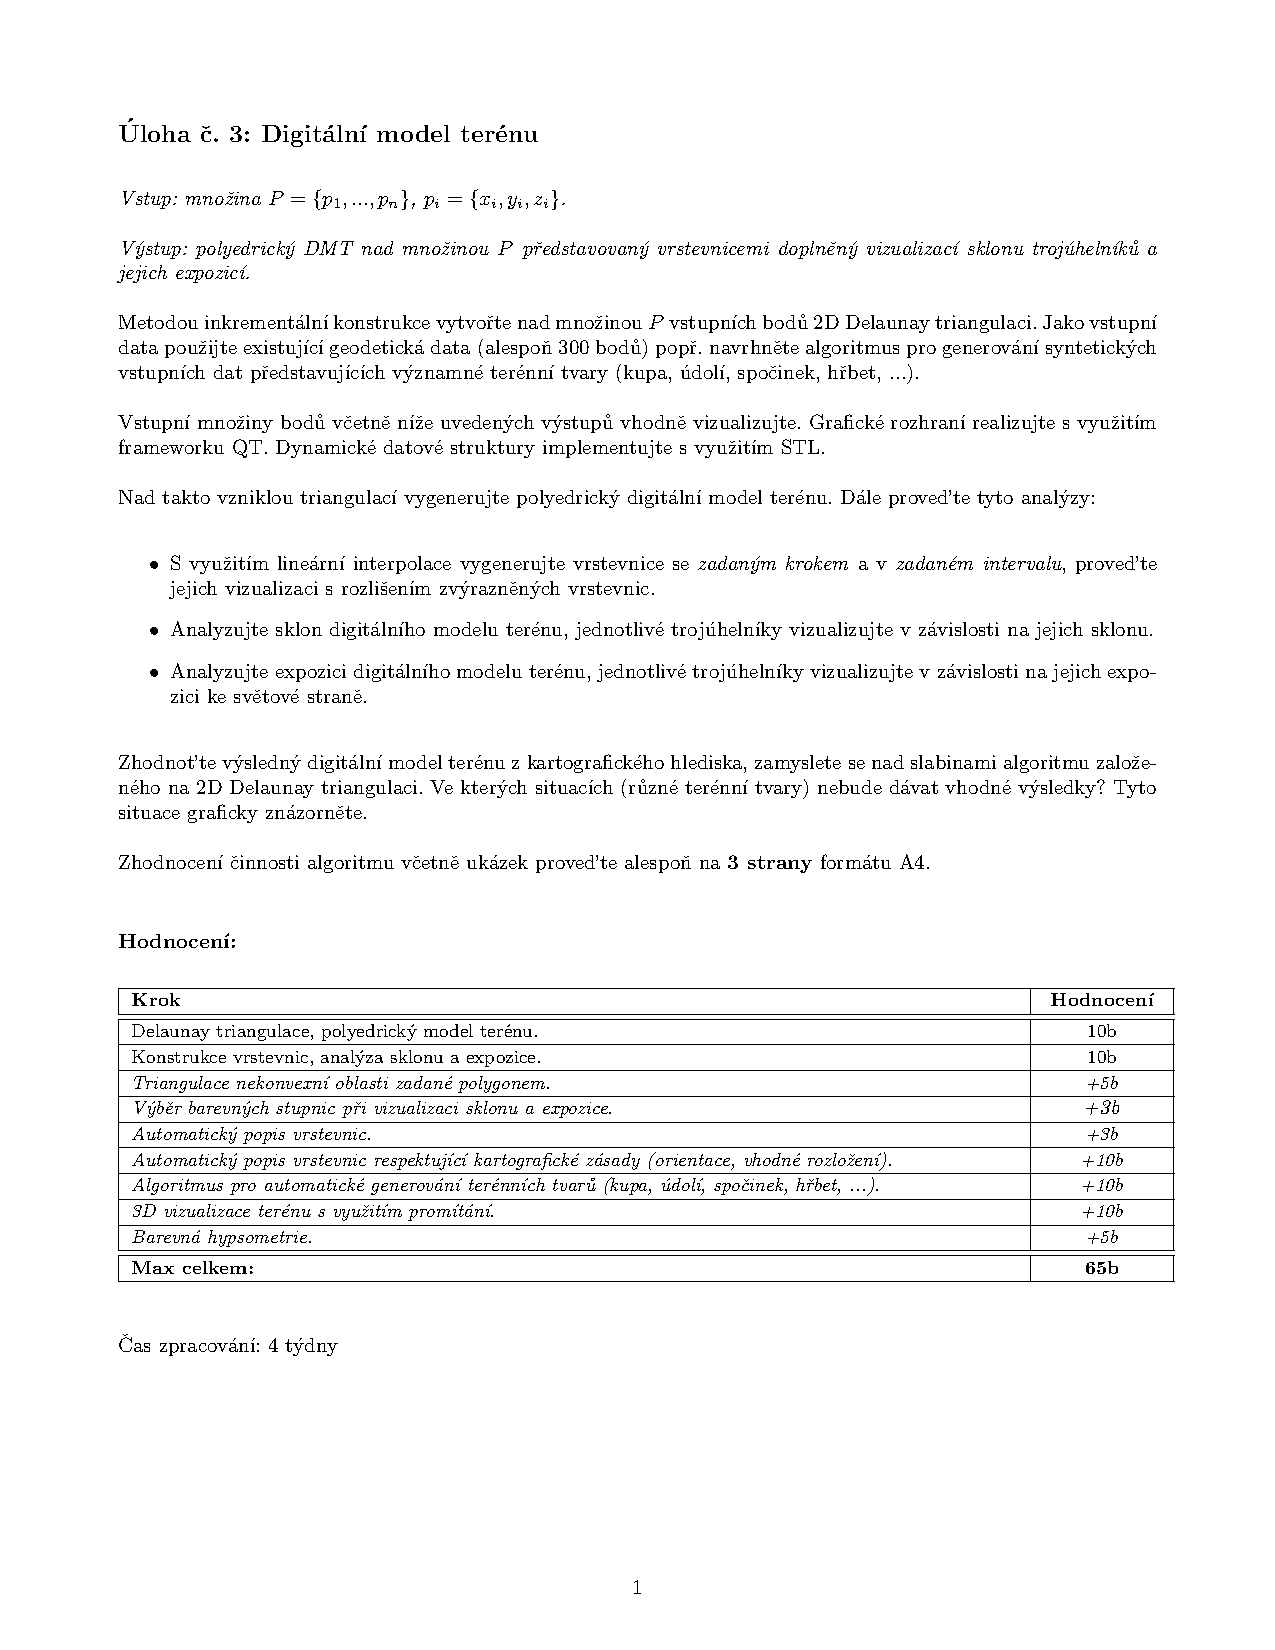
\includepdf{adkcv3}

%---------------------------------------------------------------------
\clearpage
\section{Údaje o bonusových úlohách}
\subsection{Triangulace nekonvexní oblasti zadané polygonem (+5b)}
Tato bonusová úloha nebyla řešena.

\subsection{Výběr barevných stupnic při vizualizaci sklonu a expozice (+3b)}
Byla implementována možnost výběru dvou barevných palet pro každou z vizualizací. Pro sklon terénu je možné zvolit jednu z variant "Grayscale"~--~odstíny šedé nebo "Yellow to Red"~--~žluto~--~červená paleta. Ve výběru pro expozici lze najít dvě možnosti: KM~--~zvolená námi (obr.~\ref{fig:expozice_barvy}) nebo barevnou paletu, kterou používá ArcGIS (obr.~\ref{fig:esri_expozice}). Detailnější popis je v kapitolách \ref{vyp_sklon} a \ref{vyp_exp}.


\subsection{Automatický popis vrstevnic (+3b)}
Byl implementován automatický popis hlavních vrstevnic. Hlavní vrstevnice je každá pátá vrstevnice, která je zároveň výrazněji vykreslená. Více informací je v~kapitole~\ref{popis_vrs}.

\subsection{Automatický popis vrstevnic respektující kartografické zásady (+10b)}
Tato bonusová úloha nebyla řešena.

\subsection{Algoritmus pro automatické generováních terénních tvarů (+10b)}
Bylo implementováno automatické tvoření následujících terénních tvarů: kupa, údolí, spočinek, hřbet. Zároveň je součástí aplikace možnost generování náhodných bodů. Popis řešení je v kapitole~\ref{gen_ter_tvar}.

\subsection{3D vizualizace terénu s využitím promítání (+10b)}
Tato bonusová úloha nebyla řešena.

\subsection{Barevná hypsometrie (+5b)}
Tato bonusová úloha nebyla vyřešena.


\section{Popis a rozbor problému}
Je zadaná množina bodů s~prostorovými souřadnicemi X,Y,Z. Nad těmito body je vytvořen polyedrický digitální model terénu s~využitím Delaunayho triangulace. Součástí řešení je taktéž tvorba vrstevnic, včetně jejich popisu. Dále je možné zobrazit sklon terénu (tedy sklon jednotlivých trojúhelníků v triangulaci) a expozici ke světovým stranám (rozděleno na 8 stran).


\section{Popisy algoritmů formálním jazykem} \label{popisalg}

\subsection{Delaunay triangulace} \label{dt}
Jedná se o~nejčastěji využívanou metodu triangulace. Základní funkčnost metody spočívá v~rozdělení množiny bodů tzv. Thiessenovými polygony, jejichž vlastností je ohraničení každého z~bodů vstupní množiny tak, aby z~každého místa v~ohraničeném polygonu byl nejbližším bodem právě ten ohraničený (obr.~\ref{fig:th_pol}). Hrany polygonů tvoří osu spojnice dvou bodů.

 \begin{figure}[!htb]
	\centering
	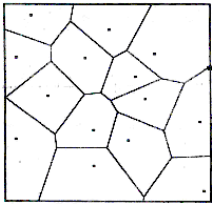
\includegraphics[scale=0.8]{obrazky/th_pol.png} 
	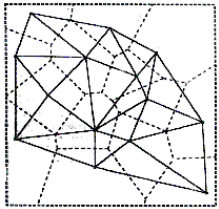
\includegraphics[scale=0.8]{obrazky/dt_obr.png}
	\caption{Ukázka Thiessenových polygonů (vlevo) a výsledné triangulace (vpravo) \cite{zcu}.
	}
	\label{fig:th_pol}
\end{figure} 
\FloatBarrier
 
Jestliže opsaná kružnice nad spojenou hranou dvou sousedních bodů neprotne jiný bod nebo jestliže se jiný bod nenachází uvnitř kružnice. Průběžným výpočtem je v~algoritmu vytvářen seznam hran (AEL~--~Active Edge List), pro které nebyl nalezen třetí bod pro triangulaci. Při nalezení nové hrany je potřeba zjistit, zda~--~se již nenachází v~AEL a tedy není případně duplicitní. Duplicitní hrany jsou odstraněny. Ve chvíli, kdy je AEL prázdný, je triangulace hotova. 

Nutné podmínky pro vytvoření triangulace:
\begin{itemize}
\item Žádný bod se nenachází uvnitř kružnice opsané libovolnému trojúhelníku triangulace.
\item Libovolné čtyři body by neměly ležet na kružnici~--~pak je triangulace nejednoznačná.
\item Maximalizace nejmenšího úhlu v trojúhelníku.
\item Splnění lokálních i globálních kritérií (vyvarování se tupých a velmi malých úhlů v~trojúhelníku, minimální suma délek stran...)
\end{itemize}

\textbf{Implementace algoritmu:} 
\begin{enumerate}
\item Nalezení náhodného a nejbližšího bodu: $p_1=rand(P), \Vert{p_1-p_2}\Vert=min.$
\item Vytvoř hranu $e=(p_1p_2)$
\item $\underline{p}=arg~min_{\forall p_i\in \sigma_L (e)}r^{'}(k_i),k_i=(a,b,p_i),e=(a,b)$
\item Pokud neexistuje $\underline{p}$, prohoď orientaci $e \leftarrow (p_2p_1)$. Jdi na 3)
\item Výpočet zbývajících hran trojúhelníka: $e_2=(p_2,\underline{p}),e_3=(\underline{p},p_1)$
\item Přidání 3 hran do AEL: $AEL \leftarrow e, AEL \leftarrow e_2, AEL \leftarrow e_3$
\item Přidání 3 hran do DT: $DT \leftarrow e, DT \leftarrow e_2, DT \leftarrow e_3$
\item Dokud AEL není prázdný:
\item \quad Vybrání první hrany z AEL: $AEL \rightarrow e, e=(p_1p_2)$
\item \quad Prohození její orientace: $e=(p_2p_1)$
\item \quad $\underline{p}=arg~min_{\forall p_i\in \sigma_L (e)}r^{'}(k_i),k_i=(a,b,p_i),e=(a,b)$
\item \quad Pokud existuje $\underline{p}$:
\item \quad \quad Zbývající hrany trojúhelníka: $e_2=(p_2,p),e_3=(\underline{p},p_1)$
\item \quad \quad Přidání hrany do DT, ale nikoliv do AEL: $DT \leftarrow e$
\item \quad \quad Přidání hrany do DT i do AEL: $add(e_2,AEL,DT), add(e_3,AEL,DT)$
\end{enumerate}

\subsection{Výpočet sklonu}\label{vyp_sklon}
Výpočet sklonu trojúhelníku je učen jako úhel~$\varphi$ mezi svislicí a normálou trojúhelníka~$n$. Výpočet probíhá vektorově nad každým z~trojúhelníků DMT. 

\begin{enumerate}
\item Určení vektorů $\overrightarrow{u}=(u_x,u_y,u_z)=(x_1-x_2, y_1-y_2, z_1-z_2), \overrightarrow{v}=(v_x,v_y,v_z)=(x_3-x_2,y_3-y_2,z_3-z_2)$ 
\item Výpočet normálového vektoru trojúhelníka: $\overrightarrow{n}=(n_y,n_y,n_z)=(u_y \cdot v_z-v_y \cdot u_z,-u_x \cdot v_z+v_x \cdot u_z,u_x \cdot v_y-v_x \cdot u_y)$
\item Sklon $\varphi =\dfrac{n_z}{\vert n\vert}$
\end{enumerate}

\subsubsection{Výběr barevné palety}
Trojúhelníky jsou vizualizovány na základě hodnoty~$\varphi$. Vizualizace je možná s~užitím dvou barevných palet. První možností jsou odstíny šedé

 \begin{figure}[!htb]
	\centering
	
\includegraphics[scale=0.11]{obrazky/gs.png} 
	
\includegraphics[scale=0.2]{obrazky/yr.png}
	\caption{Barevné palety pro vizualizaci sklonu terénu. Vlevo odstíny šedé a vpravo žluto~--~červená stupnice.
	}
	\label{fig:th_pol}
\end{figure} 
\FloatBarrier
\subsection{Výpočet expozice}\label{vyp_exp}
Výpočet expozice probíhá obdobným způsobem jako výpočet sklonu. V~podstatě jde o~úhel mezi x~--~ovou a y~--~ovou složkou normály trojúhelníka. Expozice určuje náklon trojúhelníka k jedné ze světových stran. V~aplikaci je uvažováno s~8 možnostmi (jih, jihozápad, západ, severozápad, sever, severovýchod, východ a  jihovýchod).

\begin{enumerate}
\item Určení vektorů $\overrightarrow{u}=(u_x,u_y,u_z)=(x_1-x_2, y_1-y_2, z_1-z_2), \overrightarrow{v}=(v_x,v_y,v_z)=(x_3-x_2,y_3-y_2,z_3-z_2)$ 
\item Výpočet normálového vektoru trojúhelníka: $\overrightarrow{n}=(n_y,n_y,n_z)=(u_y \cdot v_z-v_y \cdot u_z,-u_x \cdot v_z+v_x \cdot u_z,u_x \cdot v_y-v_x \cdot u_y)$
\item Určení expozice $exp=arccos\dfrac{n_z}{\vert n\vert}$
\end{enumerate}

\subsubsection{Výběr barevné palety}
Pro expozici jsou na výběr dvě možnosti barevných palet. Námi zvolená KM paleta a standardní paleta, kterou využívá např. ArcGIS.

\begin{figure}[!htb]
	\centering
	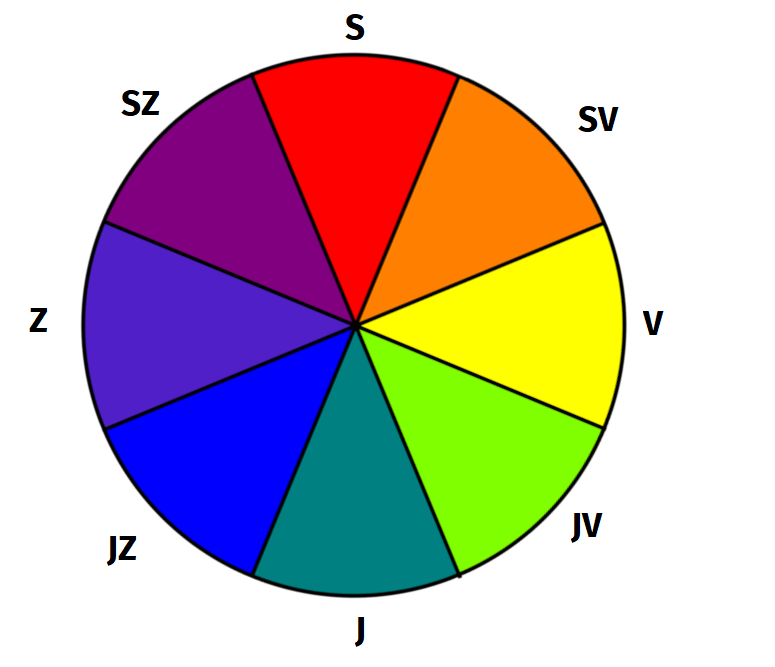
\includegraphics[scale=0.3]{obrazky/expozice_barvy.png} 
	\caption{KM barevná paleta pro vizualizaci expozice terénu.
	}
	\label{fig:expozice_barvy}
\end{figure} 
\FloatBarrier

\begin{figure}[!htb]
	\centering
	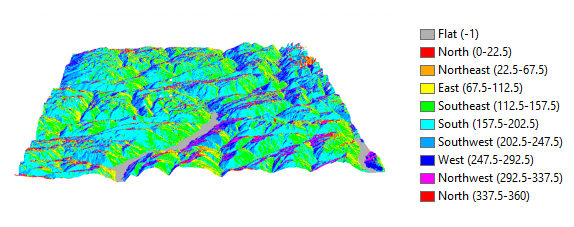
\includegraphics[scale=0.7]{obrazky/esri_expozice.png} 
	\caption{Vizualizace expozice terénu dle ArcGIS \cite{arcgispro}.
	}
	\label{fig:esri_expozice}
\end{figure} 
\FloatBarrier

\subsection{Výpočet vrstevnic}
Výpočet vrstevnic probíhá na základě vstupní Delaunayho triangulace, minimální a maximální výšky a rozestupu mezi vrstevnicemi. Jedná se o~určení vrstevnic lineární interpolací, předpoklad je tedy takový, že spád terénu je mezi podrobnými body konstantní. Jedná se o nejjednodušší a rozšířený způsob tvorby vrstevnic.

Nejprve je nutné zjistit, zda rovina $\rho$ protíná stranu $(p_i,p_{i+1})$ trojúhelníka:
\begin{enumerate}
\item Jestliže $(z-z_i)(z-z_{i+1})<0$, pak trojúhelník protíná rovinu~$\rho$ v~obecných bodech.
\item Jestliže $(z-z_i)(z-z_{i+1})>0$, pak trojúhelník neprotíná rovinu~$\rho$.
\item Jestliže $(z-z_i)(z-z_{i+1})=0$, pak jedna ze stran trojúhelníka leží v rovině~$\rho$.
\end{enumerate}

Výpočet souřadnic průsečíku A,B vrstevnice o~nadmořské výšce~$z$ s~trojúhelníkem tvořeným body 1,2,3:

\begin{center}
$x_A=\dfrac{x_3-x_1}{z_3-z_1}(z-z_1)+x_1$\\
$y_A=\dfrac{y_3-y_1}{z_3-z_1}(z-z_1)+y_1$\\
$x_B=\dfrac{x_2-x_1}{z_2-z_1}(z-z_1)+x_1$\\
$y_B=\dfrac{y_2-y_1}{z_2-z_1}(z-z_1)+y_1$\\
\end{center}

\subsubsection{Popis vrstevnice}\label{popis_vrs}
Automatický popis vrstevnic byl implementován pro každou hlavní vrstevnici (tedy každou pátou vrstevnici). Výškový údaj je vypsán nad vrstevnicí a umístěn v~polovině triangulačního trojúhelníka. 

Ve třídě Draw je implementace následovná:

\begin{verbatim}
      //Draw main contours label
       for (Edge mcl : main_contours_label)
       {
          //Start and end point of the contour edge
          QPoint3D sl_point = mcl.getStart();
          QPoint3D el_point = mcl.getEnd();

          //Get label coordintes
          QPoint3D label_point( (sl_point.x()+el_point.x())/2, 
                                (sl_point.y()+el_point.y())/2);

          //Draw Z coordinate
          QString z = QString::number(sl_point.getZ());
          qp.drawText(label_point, z);
       }
\end{verbatim}

\subsection{Generování terénních tvarů}\label{gen_ter_tvar}
Implementace algoritmů pro generování terénních tvarů a náhodných bodů, je popsána níže zvlášť pro jednotlivé případy. Uživatel může manuálně nastavit počet vygenerovaných bodů. Řešené generované terénní tvary jsou následující: náhodné body, kupa, spočinek, hřbet a údolí. Výsledné snímky obrazovky jsou v~kapitole~\ref{snimky}.

\subsection{Náhodné body}
S~využitím funkce $rand()$ jsou vygenerovány x~--~ové, y~--~ové a z~--~ové souřadnice podrobných bodů v~rámci Canvasu (plátna). Hraničními souřadnicemi jsou rozměry plátna pro X,Y a u~souřadnice~Z je jakožto horní limit brána daná výška 1000 metrů.  

\textbf{Implementace algoritmu:}
\begin{enumerate}
\item Určení souřadnic $(x_i,y_i,z_i)$ každého bodu $p_i$, přičemž $i \in (1,n)$, kde $n$ je manuálně zvolený počet bodů množiny $points$
\item \quad Výpočet $x_i=rand()~\%~width$, kde $width$ je šířka plátna
\item \quad Výpočet $y_i=rand()~\%~height$, kde $height$ je výška plátna
\item \quad Výpočet $z_i=rand()~\%~1000$, přičemž 1000 je horní limit pro výpočet nadmořské výšky
\item \quad $p_i(x_i,y_i,z_i) \rightarrow points$
\item Opakuj pro každé $i<n$
\end{enumerate}

\subsection{Kupa}\label{kupa}
S~užitím náhodných bodů z~předchozího výpočtu, kterým se přiřadí z~--~ové souřadnice dle vzdálenosti bodů od těžiště množiny bodů $points$, je vypočtena kupa. Body v~nejbližším okolí těžiště $t$ mají nejvyšší nadmořské výšky(Z) a s~rostoucí vzdáleností od těžiště nadmořské výšky úměrně klesají. Při generování bodů je použita chyba v~rámci jednotek metrů, díky které vypadá výsledek reálněji. 

\textbf{Implementace algoritmu:}
\begin{enumerate}
\item Inicializace vstupní množiny náhodných bodů $points$ o~celkovém počtu~$n$
\item Nalezení těžiště $t$ množiny podrobných bodů $points$:
\item \quad $x_t= \dfrac{\Sigma x_i}{n}$ 
\item \quad $y_t= \dfrac{\Sigma y_i}{n}$
\item \quad $z_t= 1000$, kde 1000 je maximální hodnota pro generování výšky
\item $t \rightarrow points$
\item Výpočet výšky bodů v~závislosti na rostoucí vzdálenosti od těžiště. $\forall p_i \in points$:
\item \quad $z_i=1000-d+rand()~\%~10$, kde $d$ je vzdálenost bodů $p_i$ a $t$
\end{enumerate}

\subsection{Spočinek}
Podrobné body jsou určeny náhodně, přičemž nadmořská výška je určena postupem popsaným níže. Jedná se o~generování mírného svahu. Na základě souřadnicových rozdílu každého bodu s~předposledním bodem, je určena Z-ová souřadnice. Tímto je docíleno postupného klesání nadmořské výšky směrem od hřbetnice. Závěrem je do výpočtu vložena náhodná chyba v~nadmořské výšce, jejíž velikost je v~jednotkách metrů.

\textbf{Implementace algoritmu:}
\begin{enumerate}
\item Pro množinu bodů $points$ platí: $\forall i<n$:
\item \quad $x=x_{points~i}-x_{points~n-1}$
\item \quad $y=y_{points~i}-y_{points~n-1}$
\item \quad $z=\dfrac{x+y}{250}+500$
\item \quad $points~i \leftarrow z$
\item Opakování pro $i<n$
\end{enumerate}

\subsection{Hřbet}\label{hrbet}
Výpočet podrobných bodů na hřebu vychází taktéž z~náhodných bodů. Nejprve je náhodně určen směr, kterým bude hřbet procházet (směr osy x nebo y). Na základě určení směru proběhne setřídění souřadnic bodů dle souřadnice x nebo y. Dále je určeno těžiště obdobně jako v~případě kupy (kapitola~\ref{kupa}) a výšky podrobných bodů jsou vypočteny v~závislosti na vzdálenosti těžiště s~přihlédnutím ke směru hřbetu. Při generování bodů je použita chyba v~rámci jednotek metrů, díky které vypadá výsledek reálněji. 

\textbf{Implementace algoritmu:}
\begin{enumerate}
\item Náhodné určení směru hřbetu $\rightarrow$ seřazení bodů dle určeného směru, tedy buď podle osy~x nebo dle osy~y
\item Zadání nadmořských výšek počátečnímu a koncovému bodu (pořadí dle setřídění souřadnic z~předchozího kroku)
\item Nalezení těžiště $t$:
\item \quad $x_t= \dfrac{\Sigma x_i}{n}$ 
\item \quad $y_t= \dfrac{\Sigma y_i}{n}$
\item \quad $z_t= 1000$, kde 1000 je maximální hodnota pro generování výšky
\item $t \rightarrow points$
\item Určení výšek podobných bodů $p_i$: $\forall p_i \in points $:
\item \quad Výpočet délek $d_1$(vzdálenost $p_i$ a počátečního bodu z~$points$) a $d_2$(vzdálenost $p_i$ a předposledního bodu z~$points$) 
\item \quad Pokud $d_1<d_2$:
\item \quad \quad Pak $z_i=1000-vzd(p_i,(points_{pocatecni},points_{posledni}))+rand()~\%~10$
\item \quad \quad Jinak $z_i=1000-vzd(p_i,(points_{predposledni},points_{posledni}))+rand()~\%~10$
\item Opakování pro $i<n$
\end{enumerate}

\subsection{Údolí}
Výpočetní algoritmus pro údolí je v~podstatě totožný jako v případě hřbetu (kapitola~\ref{hrbet}), jen s~rozdílem ve výpočtu nadmořských výšek podrobných bodů. Zároveň není počítáno s~hodnotami menšími než 1000, nýbrž s~hodnotami menšími než 150 z~důvodu příklonu k~realističtějšímu znázornění situace. Při generování bodů je použita chyba v~rámci jednotek metrů, díky které vypadá výsledek reálněji. 

\textbf{Implementace algoritmu:}
\begin{enumerate}
\item Náhodné určení směru hřbetu $\rightarrow$ seřazení bodů dle určeného směru, tedy buď podle osy~x nebo dle osy~y
\item Zadání nadmořských výšek počátečnímu a koncovému bodu (pořadí dle setřídění souřadnic z~předchozího kroku)
\item Nalezení těžiště $t$:
\item \quad $x_t= \dfrac{\Sigma x_i}{n}$ 
\item \quad $y_t= \dfrac{\Sigma y_i}{n}$
\item \quad $z_t= 1000$, kde 1000 je maximální hodnota pro generování výšky
\item $t \rightarrow points$
\item Určení výšek podobných bodů $p_i$: $\forall p_i \in points $:
\item \quad Výpočet délek $d_1$(vzdálenost $p_i$ a počátečního bodu z~$points$) a $d_2$(vzdálenost $p_i$ a předposledního bodu z~$points$) 
\item \quad Pokud $d_1<d_2$:
\item \quad \quad Pak $z_i=150+vzd(p_i,(points_{pocatecni},points_{posledni}))+rand()~\%~10$
\item \quad \quad Jinak $z_i=150+vzd(p_i,(points_{predposledni},points_{posledni}))+rand()~\%~10$
\item Opakování pro $i<n$
\end{enumerate}

\section{Problematické situace a jejich rozbor} \label{problemrozbor}
% (tj. simplexy) + ošetření těchto situací v kódu
\subsection{Automatické nastavení přechodné barevné stupnice mezi žlutou a červenou}
Pro zobrazení sklonu terénu byl zvolen přechod žluté do červené jako optimální varianta, nicméně vyladění správně plynule vykreslovaných barev bylo poměrně náročné k~představení. Naštěstí existují různé vizualizační online aplikace, které umí velice názorně pomoci~--~například \cite{rgbcol}.

\begin{verbatim}
void Draw::paintEvent(QPaintEvent *event)
{
...
        if (yelred == TRUE)
        {
        //Convert to color
        int col = 255 - k * slope;
        int colg = k * slope;
        QColor color(255, colg, col);

        //Set pen and brush
        qp.setBrush(color);
        qp.setPen(color);
        }
...
}
\end{verbatim}

\subsection{Správné natočení dat vůči světovým stranám}
Aplikace umí číst vstupní data v EPSG 5514 (S-JTSK / Krovak East North), s čímž se pojí nutnost přetransformovat souřadnice do místního systému plátna spolu se záměnou souřadnic, jejich natočením a určením měřítka pro rovnoměrné vykreslení dle velikosti plátna. Transformace souřadnice je v~kódu sepsána ve třídě Draw takto: 

\begin{verbatim}
void Draw::loadPoints(std::string &path, int height, int width)
{
...
    //Load data from file
    std::ifstream coords(path);

    if(coords.is_open())
    {
        while(coords >> id >> y >> x >> z)
        {
        ...
        }
        coords.close();
    }

    //Transformation coefficient
    double kx = width/fabs(x_max - x_min);
    double ky = height/fabs(y_max - y_min);

    //Scale points to the size of Canvas
    for (int i = 0; i < points.size(); i++)
    {
        double px = points[i].x();
        double py = points[i].y();

        //Rewrite coords
        points[i].setX(-kx*(py - y_max));
        points[i].setY(ky*(px - x_min));
    }
...
}
\end{verbatim}


\section{Vstupní data}
% formát vstupních dat, popis
Vstupem je textový soubor s~prostorovými souřadnicemi X,Y,Z geodetických bodů. Tyto body jsou považovány za vstupní množinu~P. Body byly získány exportem z~Digitálního modelu reliéfu 4.~generace \cite{ZABAGED} v prosředí ArcGIS~Pro \cite{arcgispro} (viz. obr. \ref{fig:arcgis_body}). Body byly následně profiltrovány z~důvodu jednoduššího a rychlejšího výpočtu aplikace.

\begin{figure}[!htb]
	\centering
	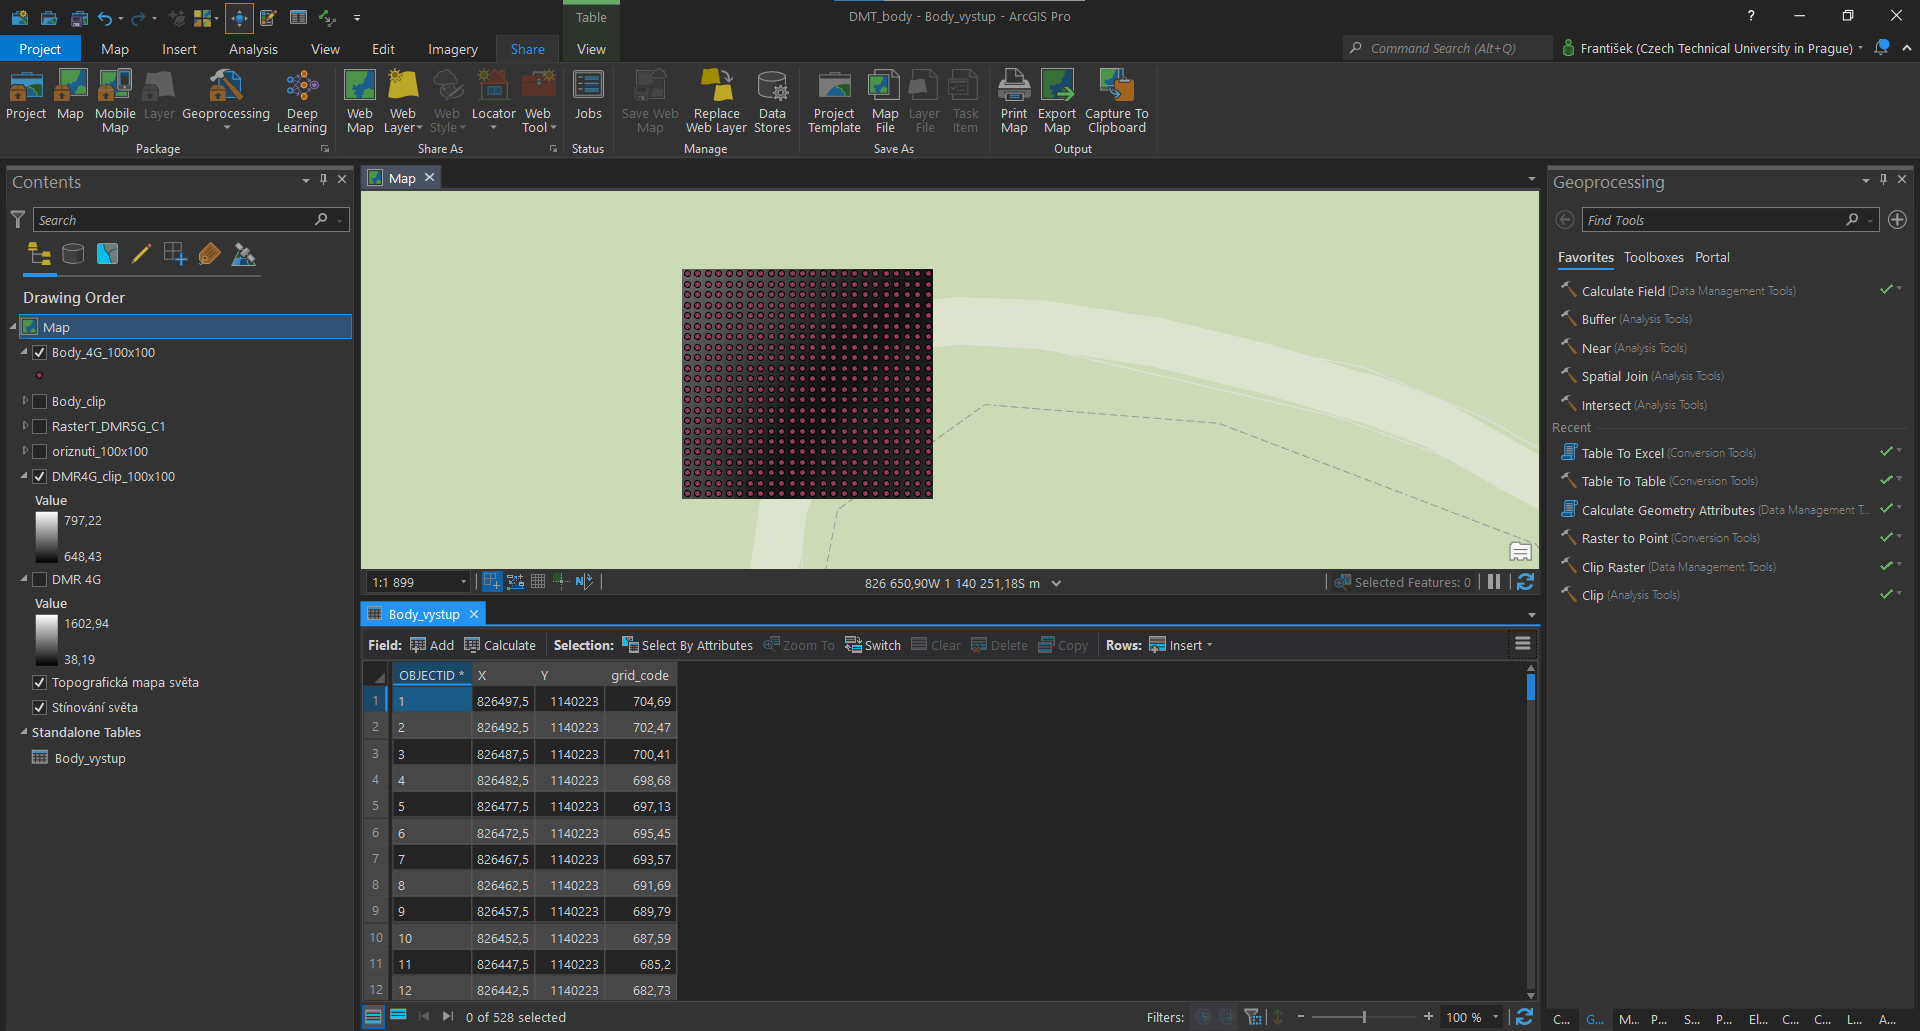
\includegraphics[scale=0.33]{obrazky/arcgis_body.png} 
	\caption{Export bodů v ArcGIS Pro z DMR4G na vybraném území.
	}
	\label{fig:arcgis_body}
\end{figure} 
\FloatBarrier

Formát vstupních dat je následující (ID, X, Y, Z):
\begin{verbatim}
1 846308.0 1129497.0 1141.2
2 846288.0 1129497.0 1131.8
3 846268.0 1129497.0 1123.2
...
\end{verbatim}


\section{Výstupní data}
% formát výstupních dat, popis
Za~výstup je považována grafický výstup vytvořené aplikace. Grafickým výstupem je polyedrický DMT nad množinou~P představovaný vrstevnicemi doplněný vizualizací sklonu trojúhelníků, jejich expozicí a vrstevnicemi s~popisem. 


\section{Snímky obrazovky vytvořené aplikace a její popis}\label{snimky}
\subsection{Popis ovládání grafického prostředí aplikace}
Grafické prostředí aplikace se skládá z~plátna, ve kterém se vykreslují grafické operace a z~nabídky funkcí aplikace v~pravé části okna. Zde se nacházejí tlačítka, rozevírací nabídky a pole pro zadání čísel. Při nesprávném použití aplikace se objeví chybová hláška s~patřičným problémem.

\textbf{Popis nabídky funkcí aplikace:} (čísla korespondují s~obr. \ref{fig:zapnuti})
\begin{enumerate}
\item Load Points načte textový soubor s podrobnými body
\item Rozevírací nabídka pro výběr generovaného terénního tvaru
\item Zadání počtu vygenerovaných bodů
\item Spuštění generování bodů
\item Vytvoření Delaunay triangulace
\item Nastavení minimální hodnoty vrstevnic
\item Nastavení maximální hodnoty vrstevnic
\item Nastavení kroku mezi vrstevnicemi
\item Spuštění kresby vrstevnic
\item Spuštění kresby popisku hlavních vrstevnic
\item Vymazání vykreslených vrstevnic
\item Výběr barevné palety pro vybarvení sklonu terénu
\item Vykreslení sklonu terénu
\item Výběr barevné palety pro vybarvení expozice částí terénu
\item Vykreslení expozice
\item Vymazání načtených bodů
\item Vymazání triangulace
\item Vymazání celého okna
\end{enumerate}

\begin{figure}[!htb]
	\centering
	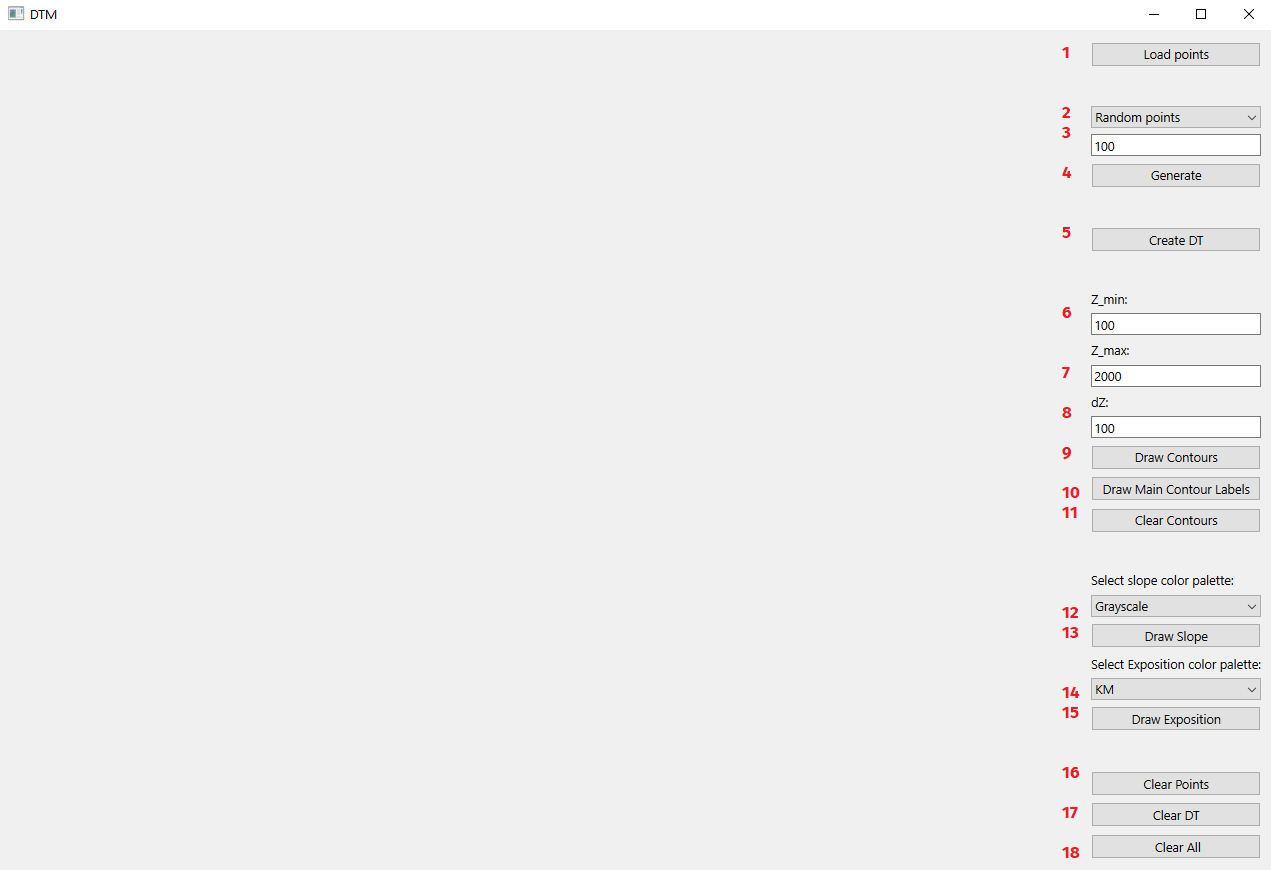
\includegraphics[scale=0.45]{obrazky/zapnuti.png} 
	\caption{Aplikace po spuštění.
	}
	\label{fig:zapnuti}
\end{figure} 
\FloatBarrier

\subsection{Vykreslení sklonu a expozice}

\begin{figure}[!htb]
	\centering
	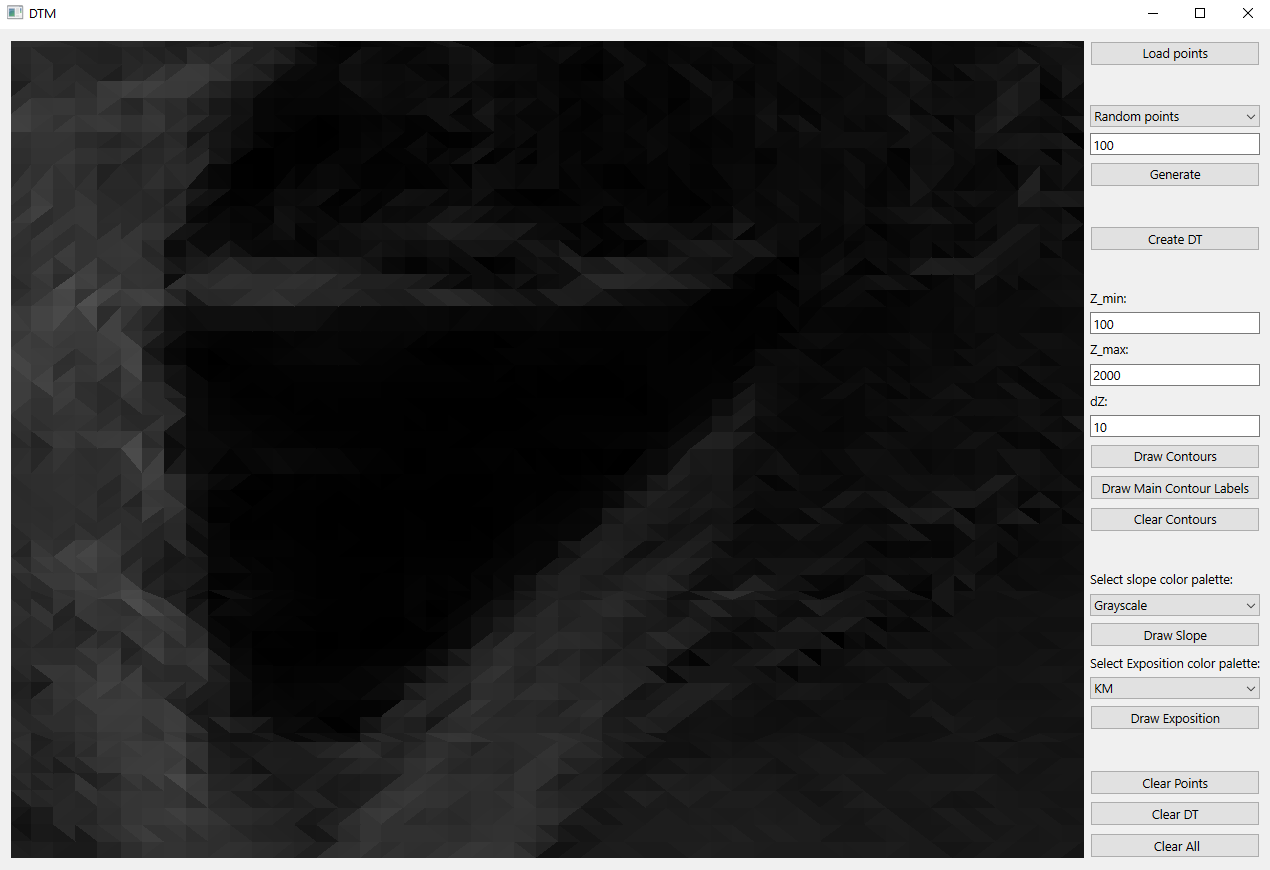
\includegraphics[scale=0.45]{obrazky/sklon_gs.png} 
	\caption{Sklon terénu v barevné paletě stupňů šedi.
	}
	\label{fig:sklon_gs}
\end{figure} 
\FloatBarrier

\begin{figure}[!htb]
	\centering
	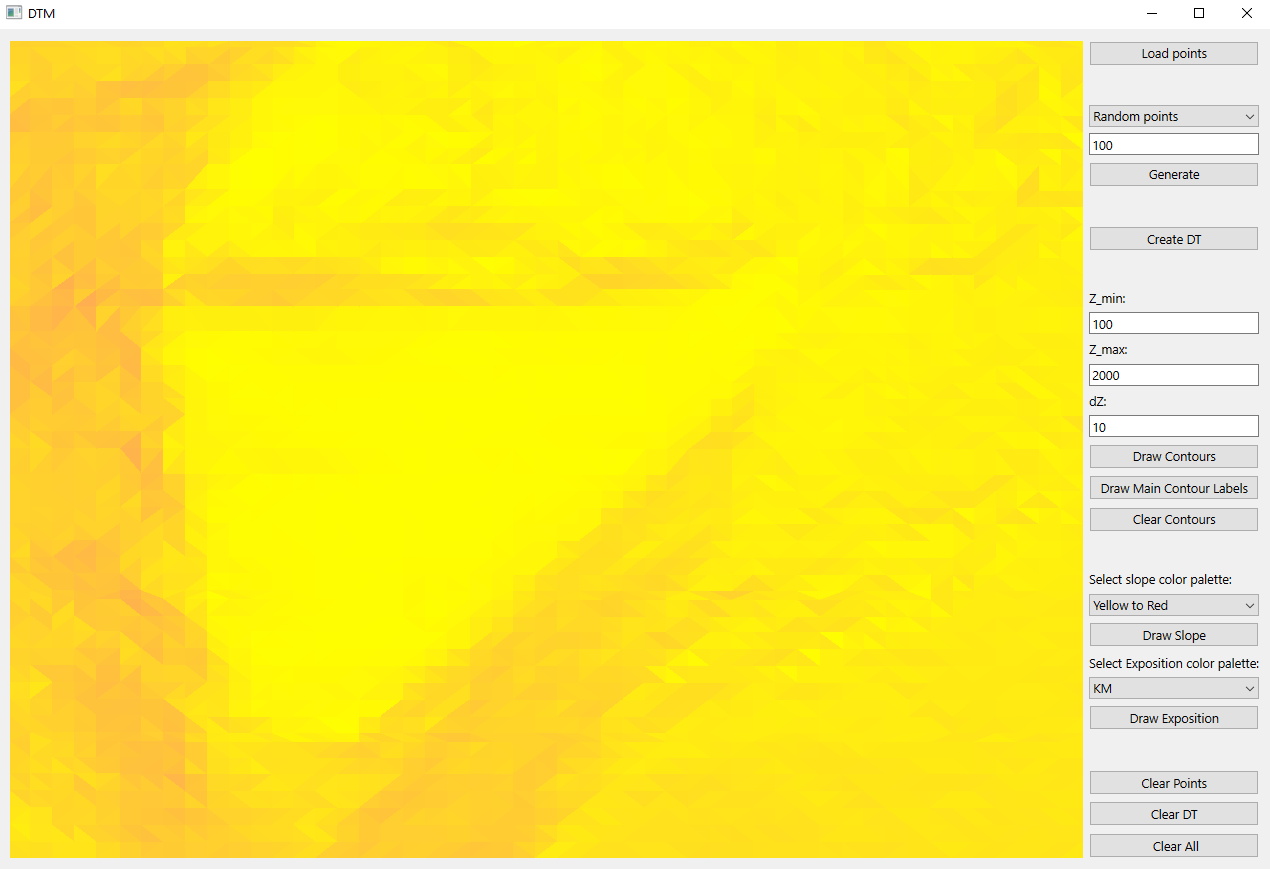
\includegraphics[scale=0.45]{obrazky/sklon_yr.png} 
	\caption{Sklon terénu ve žluto~--~červené barevné paletě.
	}
	\label{fig:sklon_yr}
\end{figure} 
\FloatBarrier

\begin{figure}[!htb]
	\centering
	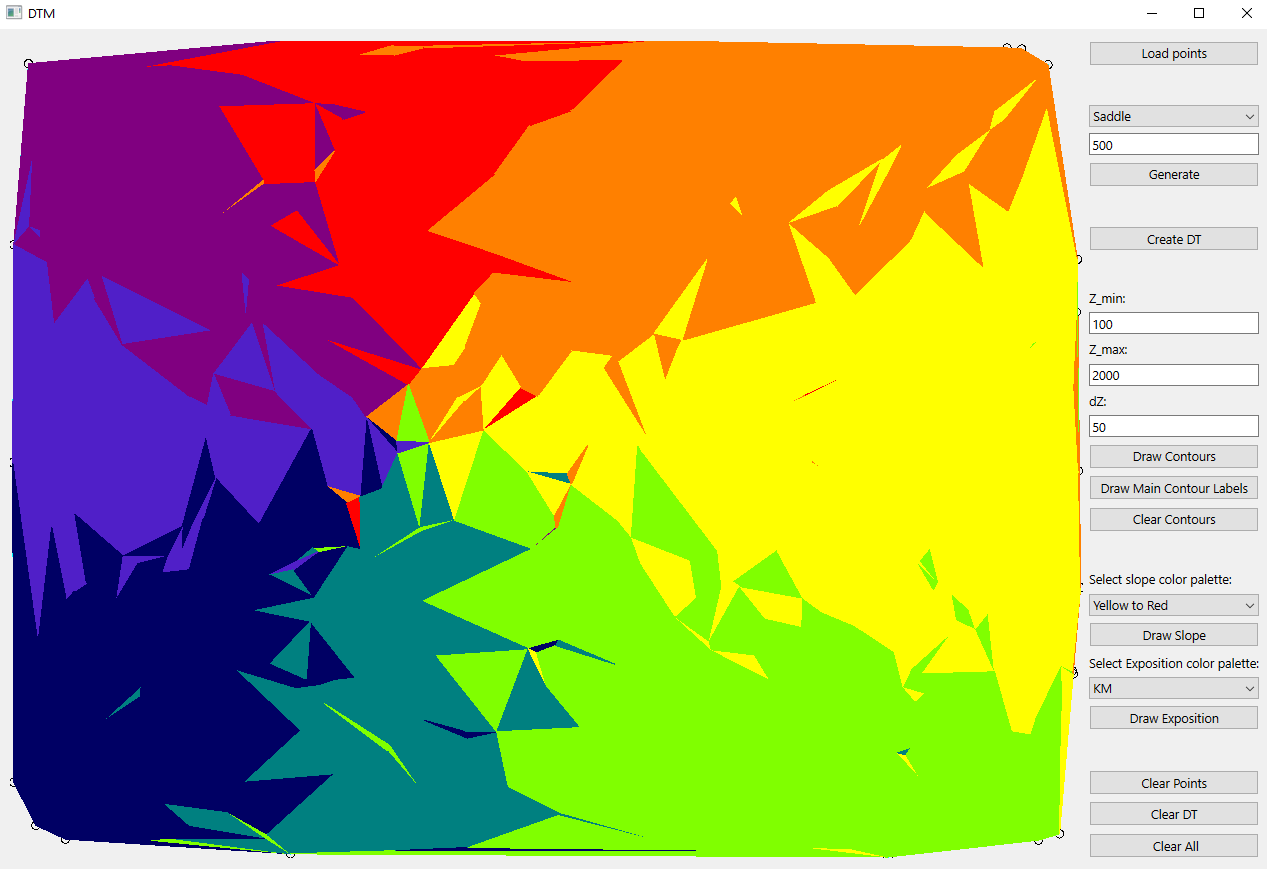
\includegraphics[scale=0.45]{obrazky/exp_km.png} 
	\caption{Expozice v KM barevné paletě.
	}
	\label{fig:exp_km}
\end{figure} 
\FloatBarrier

\begin{figure}[!htb]
	\centering
	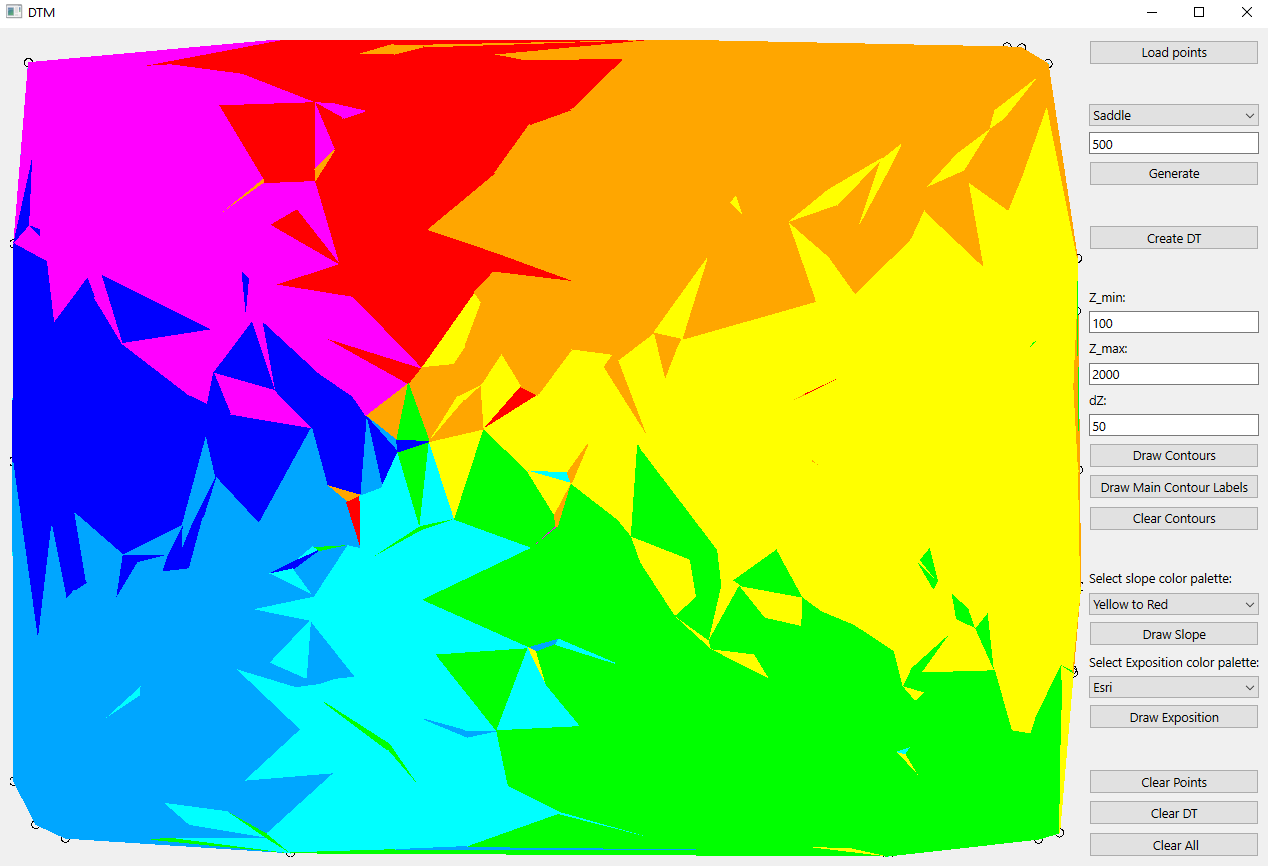
\includegraphics[scale=0.45]{obrazky/exp_arcgis.png} 
	\caption{Expozice ve standardní barevné paletě, kterou používá např. ArcGIS.
	}
	\label{fig:exp_arcgis}
\end{figure} 
\FloatBarrier

\subsection{Vykreslení vrstevnic}
\begin{figure}[!htb]
	\centering
	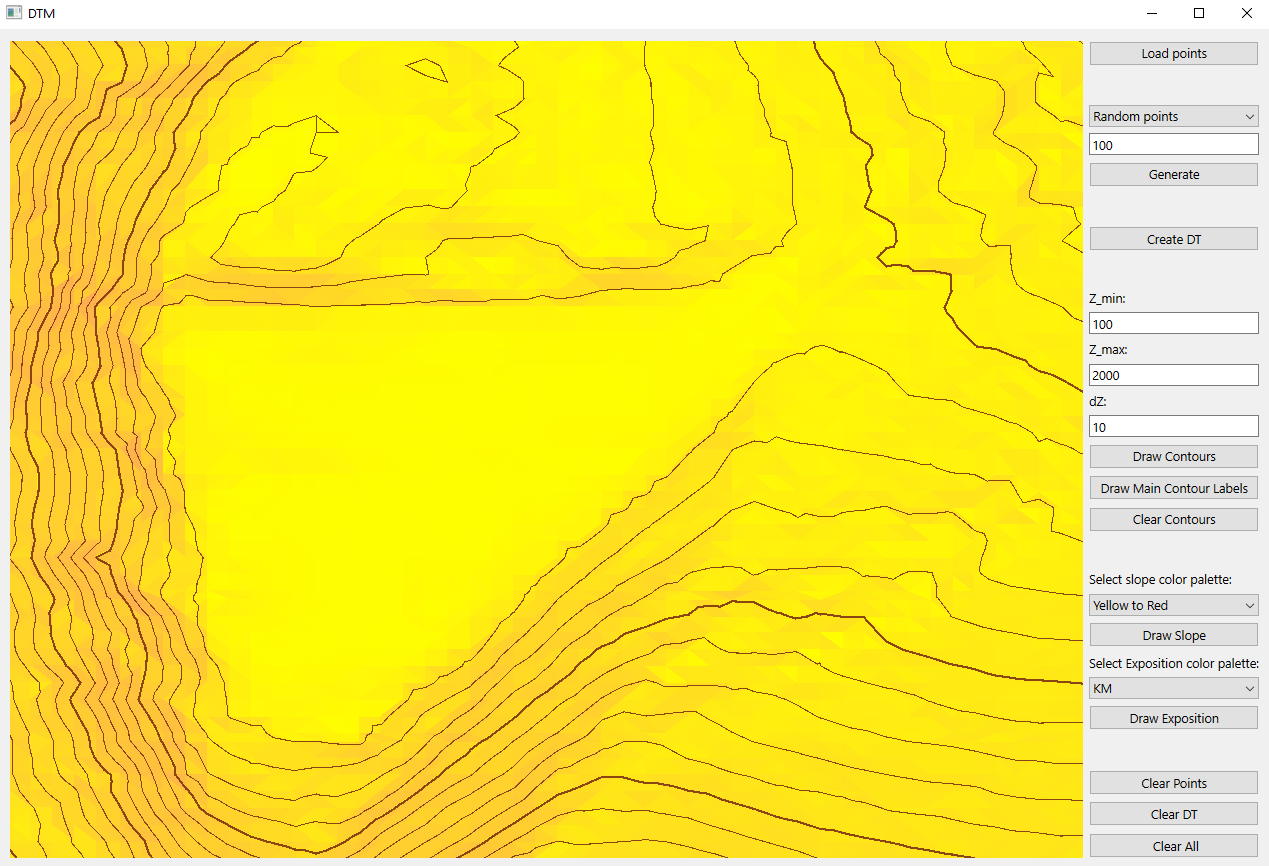
\includegraphics[scale=0.45]{obrazky/vrst_bezpop.png} 
	\caption{Vykreslení vrstevnic bez popisu.
	}
	\label{fig:vrst_bezpop}
\end{figure} 
\FloatBarrier

\begin{figure}[!htb]
	\centering
	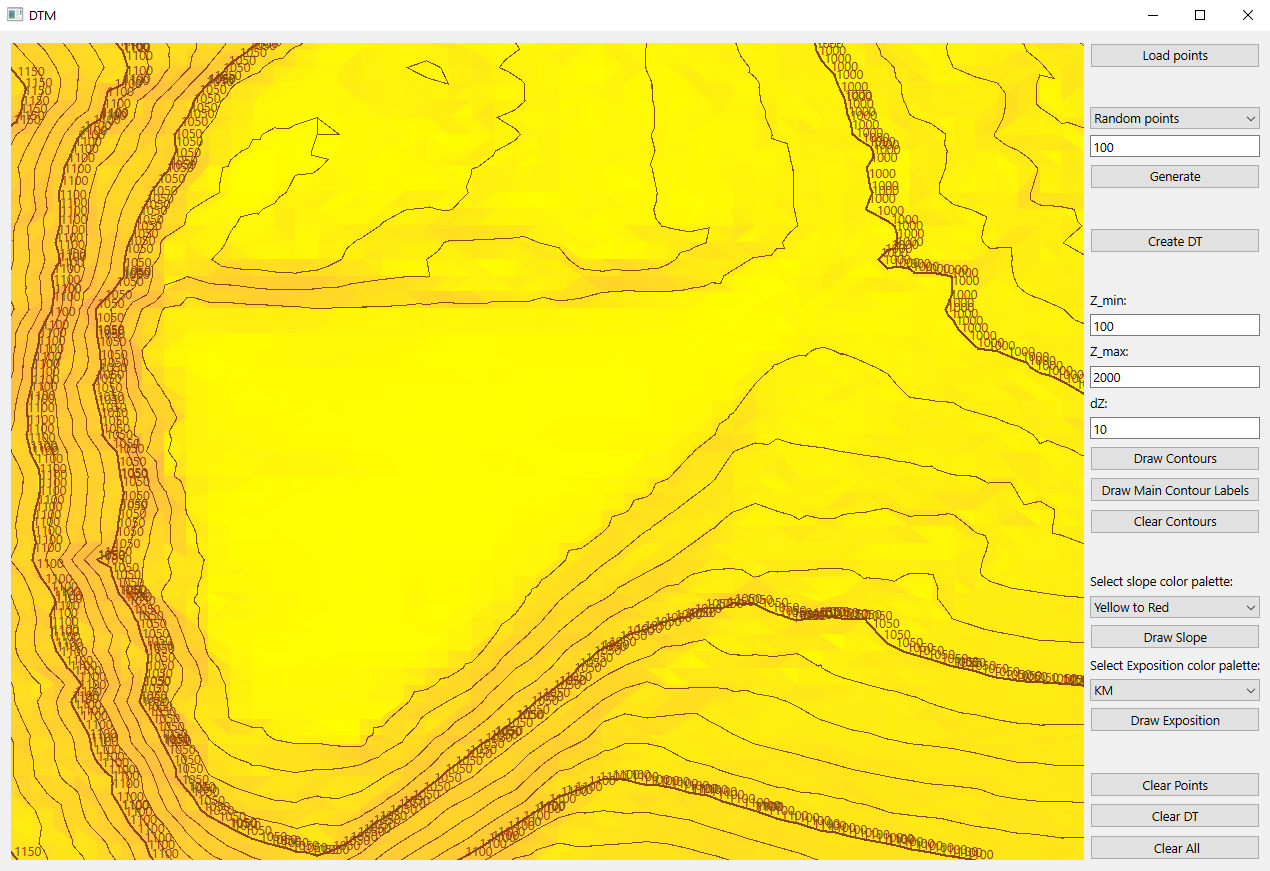
\includegraphics[scale=0.45]{obrazky/vrst_pop.png} 
	\caption{Vykreslení vrstevnic s popisem.
	}
	\label{fig:vrst_pop}
\end{figure} 
\FloatBarrier


\subsection{Generování terénních tvarů}
\begin{figure}[!htb]
	\centering
	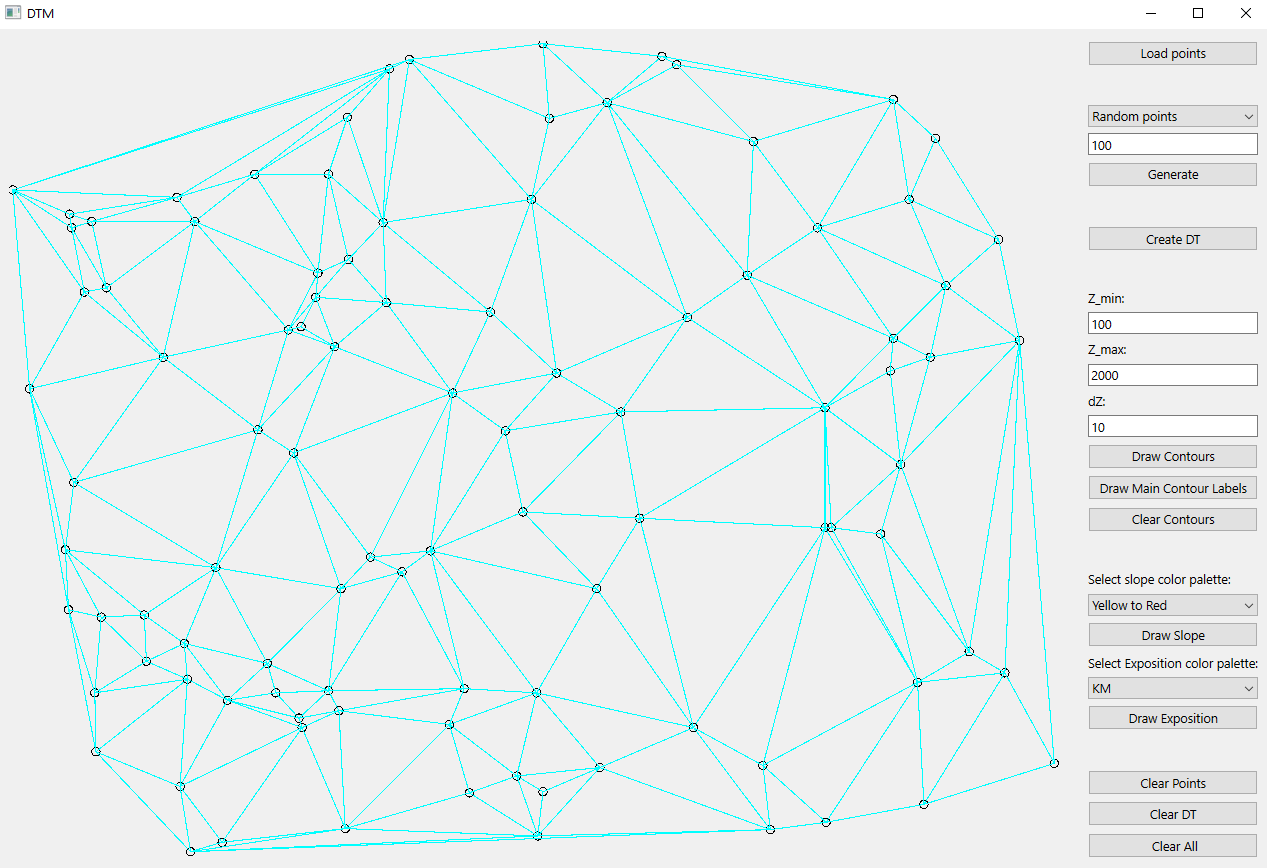
\includegraphics[scale=0.45]{obrazky/rand_dt.png} 
	\caption{Delaunay triangulace nad náhodně generovanými body.
	}
	\label{fig:rand_dt}
\end{figure} 
\FloatBarrier

\begin{figure}[!htb]
	\centering
	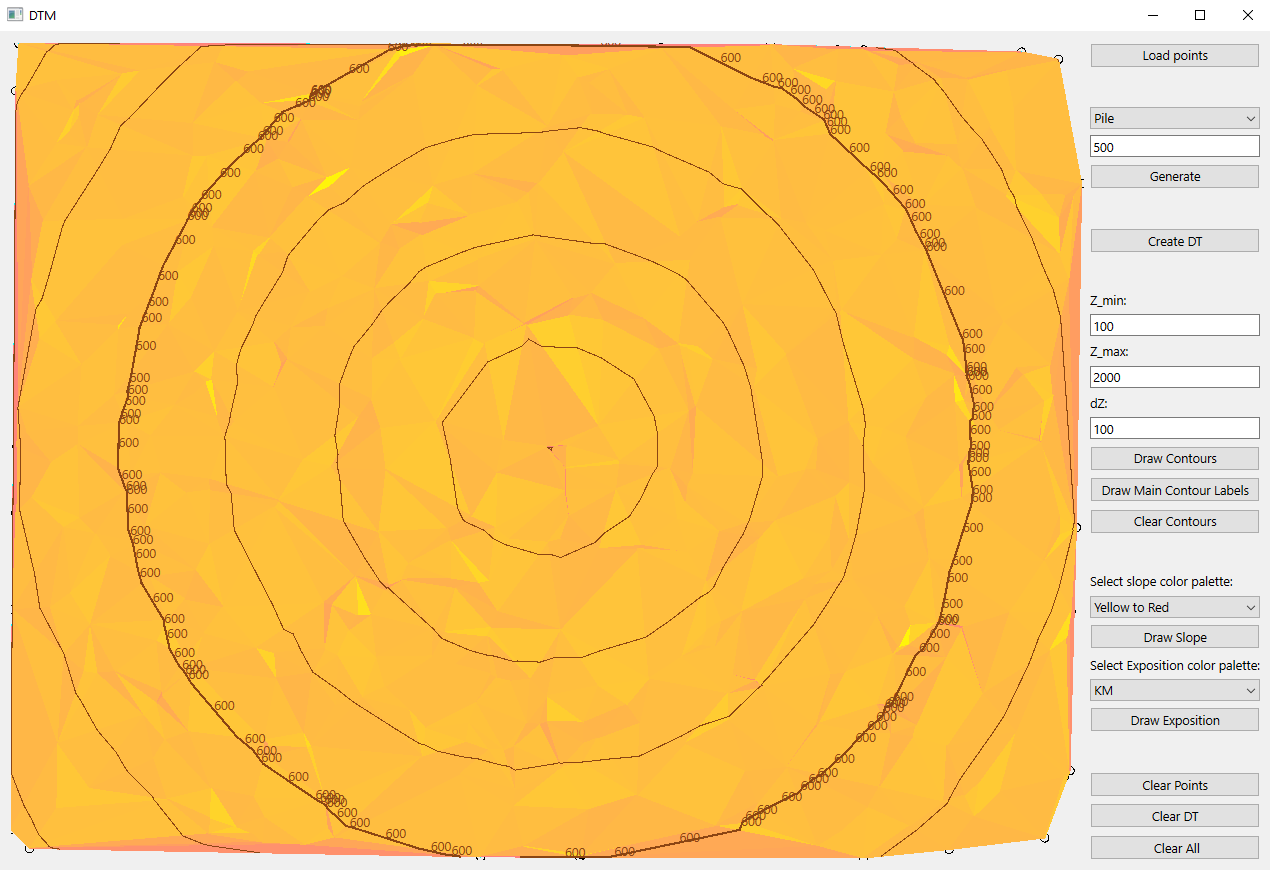
\includegraphics[scale=0.45]{obrazky/kupa.png} 
	\caption{Vykreslení kupy.
	}
	\label{fig:kupa}
\end{figure} 
\FloatBarrier

\begin{figure}[!htb]
	\centering
	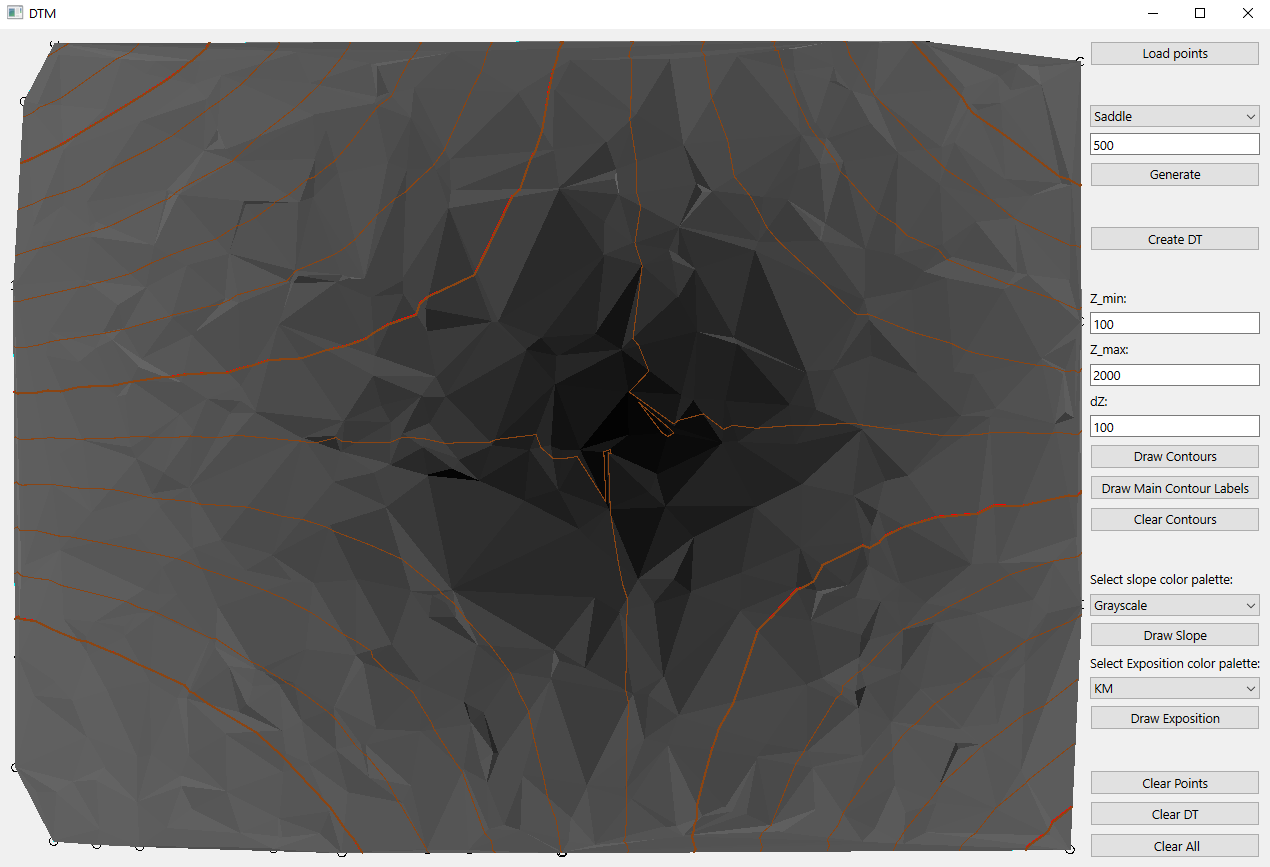
\includegraphics[scale=0.45]{obrazky/spocinek.png} 
	\caption{Vykreslení spočinku.
	}
	\label{fig:spocinek}
\end{figure} 
\FloatBarrier

\begin{figure}[!htb]
	\centering
	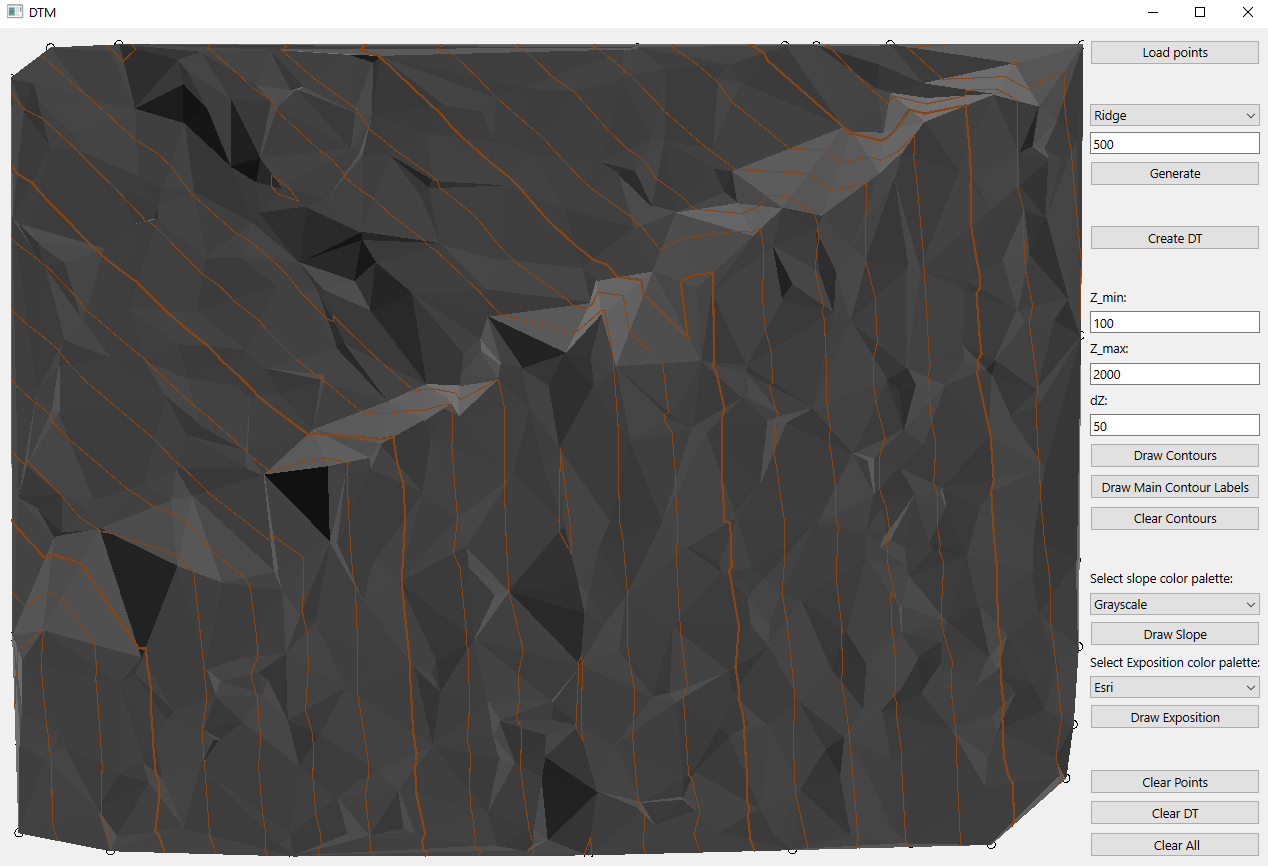
\includegraphics[scale=0.45]{obrazky/hrbet.png} 
	\caption{Vykreslení hřbetu.
	}
	\label{fig:hrbet}
\end{figure} 
\FloatBarrier

\begin{figure}[!htb]
	\centering
	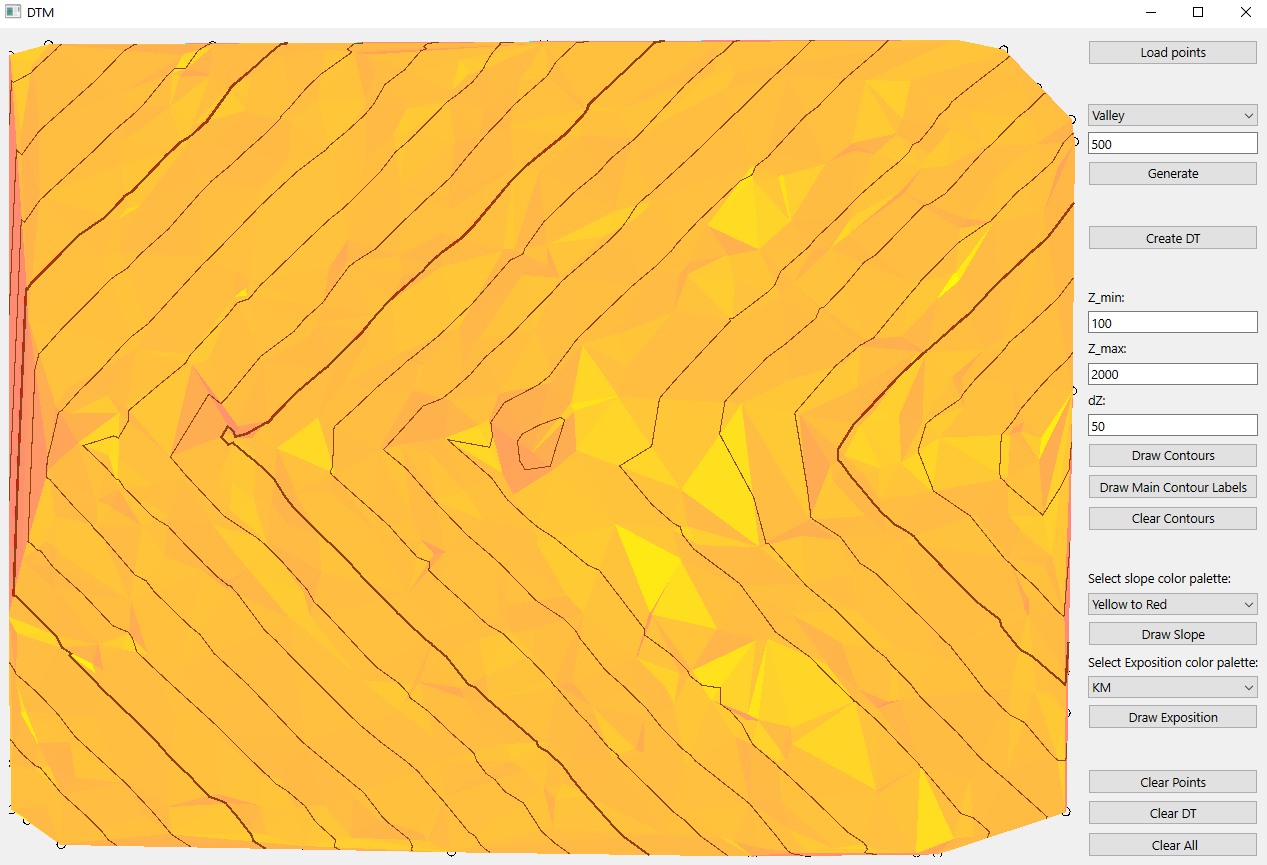
\includegraphics[scale=0.45]{obrazky/udoli.png} 
	\caption{Vykreslení údolí.
	}
	\label{fig:udoli}
\end{figure} 
\FloatBarrier

\subsection{Chybové hlášky}
\begin{figure}[!htb]
	\centering
	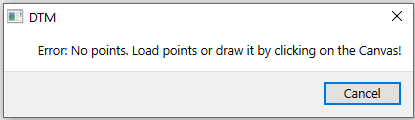
\includegraphics[scale=0.7]{obrazky/no_points.png} 
	\caption{Chyb. hl. pro nutnost načtení bodů.
	}
	\label{fig:no_points}
\end{figure} 
\FloatBarrier

\begin{figure}[!htb]
	\centering
	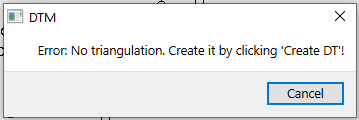
\includegraphics[scale=0.7]{obrazky/no_dt.png} 
	\caption{Chyb. hl. pro nutnost vytvoření triangulace.
	}
	\label{fig:no_dt}
\end{figure} 
\FloatBarrier

\begin{figure}[!htb]
	\centering
	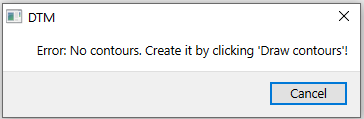
\includegraphics[scale=0.7]{obrazky/no_contours.png} 
	\caption{Chyb. hl. pro nutnost vytvoření vrstevnic.
	}
	\label{fig:no_contours}
\end{figure} 
\FloatBarrier



\section{Dokumentace}
% popis tříd, datových položek a jednotlivých metod
\subsection{Třída Algorithms}
Tato třída obsahuje výpočetní vzorce pro použité algoritmy.

\textbf{Třída algorithms obsahuje následující veřejné metody:}

\begin{verbatim}
int getPointLinePosition(QPoint &a,QPoint &p1,QPoint &p2)
\end{verbatim}
Metoda určuje, zda~--~li bod leží v~levé či v~pravé polorovině od přímky (hrany polygonu). Vstupními parametry jsou určovaný bod~$a$ a body $p_1, p_2$, které tvoří přímku.\\

\begin{verbatim}
std::tuple<QPoint3D,double> getCircleCenterAndRadius(
    QPoint3D &p1,QPoint3D &p2,QPoint3D &p3)
\end{verbatim}
Vytvoření opsané kružnice nad třemi body.\\

\begin{verbatim}
int getDelaunayPoint(QPoint3D &s,QPoint3D &e,std::vector<QPoint3D> &points)
\end{verbatim}
Určení Delaunay bodu pro triangulaci.\\

\begin{verbatim}
int getNearestPoint(QPoint3D &p, std::vector<QPoint3D> &points)
\end{verbatim}
Nalezení nejbližšího bodu.\\

\begin{verbatim}
std::vector<Edge> dT(std::vector<QPoint3D> &points)
\end{verbatim}

\begin{verbatim}
void updateAEL(Edge &e, std::list<Edge> &ael)
\end{verbatim}
Aktualizace seznamu AEL pro Delaunay triangulaci.\\

\begin{verbatim}
QPoint3D getContourPoint(QPoint3D &p1, QPoint3D &p2, double z)
\end{verbatim}
Nalezení průsečíku trojúhelníku a horizontální vrstevnice.\\

\begin{verbatim}
std::vector<Edge> getContourLines(
    std::vector<Edge> &dt, double zmin, double zmax, double dz)
\end{verbatim}
Výpočet vrstevnic na základě zadaných hran triangulace, minimální a maximální hodnoty vrstevnic a rozestupu mezi vrstevnicemi.\\

\begin{verbatim}
double getSlope(QPoint3D &p1, QPoint3D &p2, QPoint3D &p3)
\end{verbatim}
Výpočet sklonu trojúhelníka tvořeného vstupními body.\\

\begin{verbatim}
double getExposition(QPoint3D &p1, QPoint3D &p2, QPoint3D &p3)
\end{verbatim}
Výpočet expozice trojúhelníka tvořeného vstupními body.\\

\begin{verbatim}
std::vector<Triangle> analyzeDTM(std::vector<Edge> &dt)
\end{verbatim}
Výpočet sklonu a expozice pro každý trojúhelník v~triangluaci.\\

\begin{verbatim}
double distance(QPoint3D &p1, QPoint3D p2)
\end{verbatim}
Výpočet vzdálenosti mezi dvěma body.\\

\begin{verbatim}
double pointLineDistance(QPoint3D &q, QPoint3D &p1, QPoint3D &p2)
\end{verbatim}
Výpočet vzdálenosti bodu od přímky.\\

\begin{verbatim}
std::vector<QPoint3D> generateRandomPoints(int n, int height, int width)
\end{verbatim}
Generování náhodných bodů na základě jejich počtu a rozměrů plátna.\\

\begin{verbatim}
std::vector<QPoint3D> generatePile(std::vector<QPoint3D> &points)
\end{verbatim}
Generování kupy s využitím náhodných bodů.\\

\begin{verbatim}
std::vector<QPoint3D> generateSaddle(std::vector<QPoint3D> &points)
\end{verbatim}
Generování spočinku s využitím náhodných bodů.\\

\begin{verbatim}
std::vector<QPoint3D> generateValley(std::vector<QPoint3D> &points)
\end{verbatim}
Generování údolí s využitím náhodných bodů.\\

\begin{verbatim}
std::vector<QPoint3D> generateRidge(std::vector<QPoint3D> &points)
\end{verbatim}
Generování hřbetu s využitím náhodných bodů.\\

    
    
\subsection{Třída Draw}
Tato třída umožňuje vykreslování bodů, trojúhelníků a vrstevnic.

\textbf{Třída draw obsahuje následující privátní proměnné:}
\begin{verbatim}
std::vector<QPoint> points
\end{verbatim}
Proměnná se souřadnicemi načtených bodů.\\

\begin{verbatim}
std::vector<Edge> dt
\end{verbatim}
Proměnná pro ukládání hran tvořených dvěma body.\\

\begin{verbatim}
std::vector<Edge> contours, main_contours, main_contours_label
\end{verbatim}
Proměnná pro výpočet vrstevnic a jejich popisů.\\

\begin{verbatim}
std::vector<Triangle> triangles, triangles_exp
\end{verbatim}
Proměnná pro ukládání trojúhelníků tvořených třemi body.\\

\begin{verbatim}
bool grayscale, yelred, kmcol, esricol
\end{verbatim}
Proměnná pro výběr barevných palet.\\

\textbf{Třída draw obsahuje následující veřejné metody:}
\begin{verbatim}
void clear();
\end{verbatim}
Vymazání daného objektu.\\

\begin{verbatim}
void setPoints(std::vector<QPoint3D> &points_){points = points_;}
\end{verbatim}
Nastavení podrobných bodů.\\

\begin{verbatim}
std::vector<QPoint3D> getPoints(){return points;}
\end{verbatim}
Předání podrobných bodů.\\

\begin{verbatim}
void setDT(std::vector<Edge> &dt_){dt = dt_;}
\end{verbatim}
Nastavení hran Delaunay triangulace.\\

\begin{verbatim}
std::vector<Edge> getDT(){return dt;}
\end{verbatim}
Předání hran Delaunay triangulace.\\

\begin{verbatim}
void setContours(std::vector<Edge> &contours_){contours = contours_;}
\end{verbatim}
Nastavení vrstevnic.\\

\begin{verbatim}
std::vector<Edge> getContours(){return contours;}
\end{verbatim}
Předání vrstevnic.\\

\begin{verbatim}
std::vector<Triangle> getTriangles(){return triangles;}
\end{verbatim}
Předání trojúhelníků.\\

\begin{verbatim}
void setTriangles(std::vector<Triangle> &triangles_){triangles = triangles_;}
\end{verbatim}
Nastavení trojúhelníků.\\

\begin{verbatim}
void clearDT();
\end{verbatim}
Vymazání Delaunay triangulace z plátna.\\

\begin{verbatim}
void clearAll();
\end{verbatim}
Vymazání celého plátna.\\

\begin{verbatim}
std::vector<Triangle> getTrianglesExp(){return triangles_exp;}
\end{verbatim}
Předání trojúhelníků s expozicí.\\

\begin{verbatim}
void setTrianglesExp(std::vector<Triangle> &triangles_exp_)
    {triangles_exp = triangles_exp_;}
\end{verbatim}
Natavení trojúhelníků s expozicí.\\

\begin{verbatim}
void clearSlope(){triangles.clear();}
\end{verbatim}
Vymazání sklonu terénu z plátna.\\

\begin{verbatim}
void clearExposition(){triangles_exp.clear();}
\end{verbatim}
Vymazání expozice z plátna.\\

\begin{verbatim}
void clearContours(){
    contours.clear(), main_contours.clear(), main_contours_label.clear();}
\end{verbatim}
Vymazání vrstevnic z plátna.\\

\begin{verbatim}
void loadPoints(std::string &path, int height, int width)
\end{verbatim}
Načtení bodů z textového souboru.\\

\begin{verbatim}
void setMainContours(std::vector<Edge> &main_contours_)
    {main_contours = main_contours_;}
\end{verbatim}
Nastavení hlavních vrstevnic.\\

\begin{verbatim}
std::vector<Edge> getMainContours(){return main_contours;}
\end{verbatim}
Předání hlavních vrstevnic.\\

\begin{verbatim}
void setMainContoursLabel(std::vector<Edge> &main_contours_label_
    {main_contours_label = main_contours_label_;}
\end{verbatim}
Nastavení popisu hlavních vrstevnic.\\

\begin{verbatim}
std::vector<Edge> getMainContoursLabel(){return main_contours_label;}
\end{verbatim}
Předání popisu hlavních vrstevnic.\\

\begin{verbatim}
void setGrayscale(bool &grayscale_){grayscale = grayscale_;}
\end{verbatim}
Natavení šedobílé barevné palety.\\

\begin{verbatim}
void setYelRed(bool &yelred_){yelred = yelred_;}
\end{verbatim}
Nastavení žlutočervené barevné palety.\\

\begin{verbatim}
void setKMCol(bool &kmcol_){kmcol = kmcol_;}
\end{verbatim}
Nastavení první možnosti pro vykreslení expozice.\\

\begin{verbatim}
void setEsriCol(bool &esricol_){esricol = esricol_;}
\end{verbatim}
Nastavení druhé možnosti pro vykreslení expozice.\\

\subsection{Edge}
Třída uchovávající informace o hranách tvořených dvěma body.\\
\textbf{Třída draw obsahuje následující veřejné metody:}
\begin{verbatim}
void changeOrientation(){QPoint3D temp=s; s=e; e=temp;}
\end{verbatim}
Změna orientace hrany.\\

\begin{verbatim}
QPoint3D getStart() const {return s;}
\end{verbatim}
Vrácení počátečního bodu hrany.\\

\begin{verbatim}
QPoint3D getEnd() const {return e;}
\end{verbatim}
Vrácení koncového bodu hrany.\\

\subsection{QPoint3D}
\textbf{Třída draw obsahuje následující privátní proměnnou:}
\begin{verbatim}
double z
\end{verbatim}
Nadmořská výška bodu.\\

\textbf{Třída draw obsahuje následující veřejné metody:}
\begin{verbatim}
void setZ(double z_){z = z_;}
\end{verbatim}
Nastavení nadmořské výšky bodu.\\

\begin{verbatim}
double getZ(){return z;}
\end{verbatim}
Předání nadmořské výšky bodu.\\

\subsection{Třída SortByX}
\textbf{Třída draw obsahuje následující veřejnou proměnnou:}
\begin{verbatim}
bool operator() (QPoint &p1, QPoint &p2)
\end{verbatim}
Řazení bodů dle jejich x~--~ové souřadnice.\\

\subsection{Třída SortByY}
\textbf{Třída draw obsahuje následující veřejnou proměnnou:}
\begin{verbatim}
bool operator() (QPoint &p1, QPoint &p2)
\end{verbatim}
Řazení bodů dle jejich y~--~ové souřadnice.\\

\subsection{Triangle}
Třída tvořící trojúhelník.\\
\textbf{Třída draw obsahuje následující privátní proměnné:}
\begin{verbatim}
QPoint3D p1, p2, p3
\end{verbatim}
Vrcholy trojúhelníka.\\

\begin{verbatim}
double slope, exposition
\end{verbatim}
Sklon a expozice trojúhelníka.\\

\textbf{Třída draw obsahuje následující veřejné metody:}
\begin{verbatim}
QPoint3D getP1(){return p1;}
\end{verbatim}
Vrácení souřadnic vrcholu 1.\\

\begin{verbatim}
QPoint3D getP2(){return p2;}
\end{verbatim}
Vrácení souřadnic vrcholu 2.\\

\begin{verbatim}
QPoint3D getP3(){return p3;}
\end{verbatim}
Vrácení souřadnic vrcholu 3.\\

\begin{verbatim}
double getSlope(){return slope;}
\end{verbatim}
Předání sklonu trojúhelníka.\\

\begin{verbatim}
double getExposition(){return exposition;}
\end{verbatim}
Předání expozice trojúhelníka.\\

\begin{verbatim}
void setP1(QPoint3D &p1_){p1 = p1_;}
\end{verbatim}
Nastavení vrcholu 1.\\

\begin{verbatim}
void setP2(QPoint3D &p2_){p2 = p2_;}
\end{verbatim}
Nastavení vrcholu 2.\\

\begin{verbatim}
void setP3(QPoint3D &p3_){p3 = p3_;}
\end{verbatim}
Nastavení vrcholu 3.\\

\begin{verbatim}
void setSlope(double &slope_){slope = slope_;}
\end{verbatim}
Natavení sklonu trojúhelníka.\\

\begin{verbatim}
void setExposition(double &exposition_){exposition = exposition_;}
\end{verbatim}
Nastavení expozice trojúhelníka.\\


\subsection{Třída Widget}
Tato třída propojuje uživatelské rozhraní aplikace s kódem. Je vytvořena v sekci \emph{Design}.

\textbf{Třída widget obsahuje následující privátní metody:}
\begin{verbatim}
void on_pushButton_clearPoints_clicked()
\end{verbatim}
Vymazání podrobných bodů z plátna.\\

\begin{verbatim}
void on_pushButton_cleardt_clicked()
\end{verbatim}
Vymazání triangulace z plátna.\\

\begin{verbatim}
void on_lineEdit_editingFinished()
\end{verbatim}
Manuální zápis minimální hodnoty pro vrstevnice.\\

\begin{verbatim}
void on_lineEdit_2_editingFinished()
\end{verbatim}
Manuální zápis maximální hodnoty pro vrstevnice.\\

\begin{verbatim}
void on_lineEdit_3_editingFinished()
\end{verbatim}
Manuální zápis rozestupu mezi vrstevnicemi.\\

\begin{verbatim}
void on_pushButton_drawContours_clicked()
\end{verbatim}
Vykreslení vrstevnic.\\

\begin{verbatim}
void on_pushButton_drawSlope_clicked()
\end{verbatim}
Vykreslení sklonu terénu.\\

\begin{verbatim}
void on_pushButton_ClearAll_clicked()
\end{verbatim}
Vymazání celého plátna.\\

\begin{verbatim}
void on_pushButton_Exposition_clicked()
\end{verbatim}
Vykreslení expozice terénu.\\

\begin{verbatim}
void on_pushButton_LoadPoints_clicked()
\end{verbatim}
Načtení textového souboru se vstupními body.\\

\begin{verbatim}
void on_pushButton_mcLabels_clicked()
\end{verbatim}
Vykreslení popisů vrstevnic.\\

\begin{verbatim}
void on_pushButton_Generate_clicked()
\end{verbatim}
Generování náhodných bodů či terénních útvarů.\\

\begin{verbatim}
void on_pushButton_clearContours_clicked()
\end{verbatim}
Vymazání vrstevnic z plátna.\\

\begin{verbatim}
void on_pushButton_createDT_clicked()
\end{verbatim}
Vykreslení Delaunay triangulace.\\

\section{Závěr}
Byla vytvořena desktopová aplikace s~interaktivním grafickým prostředí, která uživateli umožňuje vypočítat a vykreslit digitální model terénu nad zadanými či náhodně generovanými bodovými daty. Je na výběr z~následujících náhodně generovaných terénních tvarů: kupa, údolí, spočinek, hřbet nebo znázornění bodů čistě náhodných. 

V aplikaci je možné vykreslit sklon terénu a expozici částí terénu k jednotlivým světovým stranám, přičemž pro obě z~možností jsou na výběr dvě barevné vykreslovací palety. Aplikace dále umožňuje vykreslení vrstevnic, včetně zvýraznění a popisu hlavních vrstevnic. Rozestup vrstevnic, včetně minimální a maximální výšky vrstevnic, lze manuálně měnit v~okně aplikace. Není implementován popis vrstevnic respektující kartografické zásady. Vývoj aplikace proběhl v~programovacím jazyce C++. 

\subsection{Zhodnocení}
Výsledný model terénu slouží jako poměrně kvalitní náhled nad načtenými daty, nicméně bez dalších úprav má stále velké nedostatky. Mezi hlavní problém jistě patří absence povinných hran, díky které se vrstevnice tvoří například po vodní ploše, jak je vidět na ukázce Černého jezera na obr.~\ref{fig:vrst_bezpop}. 

Další problematické situace nastávají při generování hřbetu a údolí. Vrstevnice v~okolí hřbetnice, respektive údolnice, tvoří jednotlivé "vrcholky" (obr.~\ref{fig:chyba_hrbet}), což by mohlo být pro uživatele matoucí při chápání mapy a zároveň tyto útvary zahlcují mapu. Bylo by tedy vhodné vykreslovat vrstevnice jen nad určitou délku.

 \begin{figure}[!htb]
	\centering
	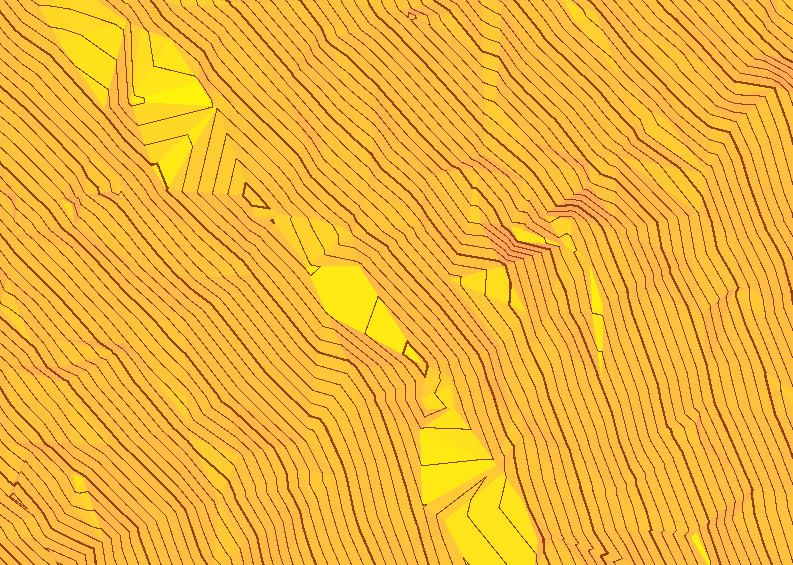
\includegraphics[scale=0.8]{obrazky/chyba_hrbet.png} 
	\caption{Chyba při generování hřbetu.
	}
	\label{fig:chyba_hrbet}
\end{figure} 
\FloatBarrier

Nicméně přes určité nedostatky se ukazuje, že užití 2D triangulace je vhodné pro prvotní náhled nad daty. Uživatel získá hrubé povědomí o~povrchu terénu a jeho členitosti. Pro pokročilejší analýzy nebo přesnější výstupy je žádoucí další úprava algoritmu a odstranění nedostatků.

\subsection{Možné či neřešené problémy} \label{mcn_problemy}
Nebyly řešeny některé bonusové úlohy. Problém může nastávat při větším objemu vstupních dat, už při 2500 vstupních bodech není triangulace rozhodně "instantní". 
Při aplikaci nad reálnými daty je objevují nedostatky výpočtu, například kreslení vrstevnic přes vodní plochu.

\subsection{Náměty na vylepšení} \label{vylepseni}
Aplikaci lze jistě vylepšit v mnoha ohledech. Grafické zpracování by mohlo být pokročilejší, bylo by možné přidat více barevných palet nebo při výběru barevné palety zobrazit její barvy, aby je uživatel znal dopředu. 
Pro zadaná data by mohla aplikace rozpoznat minimální a maximální nadmořskou výšku, a tedy by jí nemusel uživatel manuálně zadávat.




\begin{flushright}
V Praze 5. 12.2021\\
\vspace{2mm}
Bc. Pane Kuzmanov\\
Bc. František Mužík\\
\end{flushright}


%---------------------------------------------------------------------
\clearpage 
\section*{Použitá literatura}
\renewcommand{\section}[2]{}%
\bibliographystyle{acm}
\bibliography{Literatura_u3_adk}


\end{document}
